\chapter{Sparsity Tracing via NaN-Propagation}
\label{sec:nan_propagation}

A key challenge in applying code transformations is handling external black-box (i.e., non-traceable) function calls within the analysis graph. While code transformations can apply techniques like automatic differentiation and automated sparsity detection to accelerate traceable code, these efficiency gains are lost when opaque black-box functions are present. Here, gradient calculation methods must invariably fall back to slower techniques, such as finite-differencing or complex-step derivative computation \cite{martins_complexstep_2003}. The end result is that patching a black-box model into a code-transformations-based MDO tool using simple finite-differencing usually leads to poor performance.

To take a first step towards improving black-box handling in code transformation frameworks, we can ask ourselves what the minimum amount of information needed to achieve meaningful acceleration on black-boxes would be. In an ideal case, we would like to have a fast way to directly evaluate the Jacobian of the black-box function at some given point in the input space. This would allow the black-box function to be directly patched into the computational graph as its own primitive operator. Unfortunately, though some black-box functions provide direct gradient information, most do not.

If we accept that the Jacobian of a black-box function will need to be computed with finite differencing to support gradient-based optimization, the next-best option would be to obtain information that allows us to compute this faster. One example of such information is the sparsity pattern of the Jacobian of the black-box function. This sparsity pattern essentially gives a map of which inputs have the potential to affect each output. Armed with this information, we can perform Jacobian compression via coloring \cite{gebremedhin_efficient_2009, gebremedhin_what_2005, martins_engineering_2021}. This allows the Jacobian to be calculated with fewer function evaluations, even in the case of simple finite-differencing.


\section{Existing Approaches}
\label{sec:nan-existing-methods}

Currently, the most common approach to obtain the sparsity pattern of a black-box function is a \emph{gradient-based} method. First, the (dense) Jacobian is constructed via finite differencing, evaluated at some particular point in the input space that is assumed to be representative. (In the context of an optimization framework, this input point usually corresponds to the initial guess.) Then, a critical assumption is made: it is assumed that any zero entries in this evaluated Jacobian are indicative of a zero entry in the true Jacobian -- in other words, sparsity seen at one point indicates sparsity at all points. Due to this assumption, the sparsity pattern constructed with this method is only an estimate, not a guarantee.

The fact that this reconstructed sparsity pattern is only an estimate is inevitable for black-box functions. To illustrate why, consider a piecewise function, where input $x_j$ influences output $f_i$ when $x_j$ is within a certain interval but not outside of it. It is possible to construct a pathological black-box function where this region of influence is arbitrarily small, such that it will nearly never be detected by direct sampling of the Jacobian. Such cases will result in a \emph{false negative} in the estimated sparsity pattern: cases where $x_j$ and $f_i$ are believed to be independent, when in reality they are not.

This kind of branching code execution is perhaps the most common cause of such false negatives (often via conditional expressions) in the context of engineering analysis. However, there are other relevant failure modes as well. One possible cause of false negatives is if the representative input point yields a partial derivative of zero only due to coincidence, rather than due to mathematical structure. One simple illustrative example is the function $f(x) = x^2$, if the evaluation point of $x = 0$ is chosen. Here, a central finite difference will see zero gradient and incorrectly infer no dependency. On most functions of practical interest, such points are usually rare within the input space\footnote{In most practical functions $\vec{f}(\vec{x}): \R^m \rightarrow \R^n$, the dimensionality of all manifolds where $\partial f_i/\partial x_j=0$ is less than the dimensionality of the input $\vec{x}$. In such cases, \emph{almost all} points will be free of coincidental zeros.}. However, in an optimization context, the distribution of user-specified initial guesses is not uniform, and in fact adversarial: users will preferentially supply near-optimal initial guesses, which have near-zero gradients (if the problem is unconstrained). Because of this, and as demonstrated later in Section \ref{sec:nan-comparison}, this effect can contribute to a non-negligible rate of false negatives in practice.

\emph{False positives}, where $x_j$ and $y_i$ are believed to be related when they are not, are also possible, though rarer. A practical example where this could occur is with a black-box function that has truncation error, perhaps due to a nonlinear solver or numerical integrator that uses a value-dependent convergence criteria. In such cases, changing one input may alter the number of iterations required for convergence. This can cause changes in the truncation error of all outputs—even those that are mathematically-unrelated to that input. Thus, changes in this truncation error (i.e., a differing number of iterations) may yield a nonzero Jacobian entry, even if the math that the code aims to represent has no such dependency. Other false positive scenarios, such as stochastic functions, are possible but relatively uncommon in engineering analysis. In either the false-negative or false-positive case, an interesting observation is that the sparsity of the function \emph{in code} may not match the sparsity of the mathematical model the code aims to represent.

For reasons related to Jacobian compression (described later via demonstration in Section \ref{sec:nan-jacobian-compression}), the harm caused by a false-negative and a false-positive are very unequal -- false negatives are far worse. The ultimate effect of a false-positive is that subsequent gradient calculations will be slightly slower, though still numerically correct. On the other hand, the ultimate effect of a false-negative is that gradient calculations can be incorrect, due to erroneous Jacobian compression. Worse yet, these incorrect results can occur silently. In the context of design optimization, an incorrect gradient might only be detected much later in the development effort, when an optimizer consistently cannot converge (as the KKT conditions cannot be satisfied). By this point in the code development process, the combined optimization model is usually much more complex, and finding and eliminating an incorrect-gradient error becomes enormously tedious. Because of this, a new method for black-box sparsity estimation that eliminates false-negative failure modes offers significant value to the end-user, even if it comes at the cost of false-positive failure modes. In other words, the focus of black-box sparsity estimation within this context should be to build up a \emph{conservative} estimate of the sparsity pattern that trades away specificity in favor of sensitivity.


\section{NaN-Propagation Overview and Demonstration}
\label{sec:nan-demo}

This thesis contribution introduces a novel technique that we call \textit{NaN propagation} to trace these input-output dependencies through black-box functions. The name refers to ``not-a-number'' (NaN), which is a special value in floating-point arithmetic that is often used to represent undefined, missing, or otherwise unrepresentable values. The proposed technique exploits the fact that Not-a-Number (NaN) values are universally propagated through floating-point numerical computations; colloquially, they tend to ``contaminate'' any calculation that is given a NaN input. For example, a dyadic\footnote{referring to a function that accepts two input parameters} operation with a just one NaN operand will return NaN. This behavior is explicitly part of math library APIs that follow the IEEE 754 standard \cite{ieee754}, first established in 1985. Because nearly all floating-point math libraries created since the advent of IEEE 754 follow it, this presents a fascinating way to potentially trace sparsity in a way that is essentially independent of math library or programming language. By systematically contaminating inputs to a black-box function with NaN values and observing which outputs become NaN, an estimate of the sparsity pattern can be reconstructed.

As a high-level comparison against the existing technique described in this section, this proposed new technique:

\begin{itemize}[noitemsep]
    \item Eliminates a false-negative failure mode, namely coincidental zero gradients.
    \item Adds a new false-positive failure mode, for functions with internal mathematical cancellation.
    \item Is either equivalent in runtime speed, or potentially much faster due to \emph{short-circuiting operators}. This consideration is primarily determined by behavior of the math library used by the black-box function.
    \item Is compatible with most black-box functions, but not all, due to possible internal handling of NaN values. However, this incompatibility is usually easily and immediately detected, allowing the user to fall back to the existing technique.
\end{itemize}

This new technique, and strategies and mitigations around these four high-level tradeoffs, are the focus of the remainder of this chapter.

\subsection{Example Black-Box Function: Wing Weight Model in TASOPT}

Some of the more nuanced details of the proposed NaN-propagation technique are most clearly explained through demonstration. To do this, we leverage one of the constituent submodels within \emph{TASOPT}, an aircraft design optimization suite for tube-and-wing transport aircraft developed by Drela \cite{drela_tasopt_2010}. The submodel we use is a wing weight model \footnote{In TASOPT, this model is named \texttt{surfw}.}, with the major modeling considerations shown in Figure \ref{fig:nan-tasopt-wing-weight}. The model is relatively detailed, with 38 inputs and 37 outputs. Inputs include geometric parameters, material properties, and configuration-level decisions (e.g., the number and location of engines, or the presence and dimensions of a strut). Outputs are the weights of various wing components, metrics describing the weight distribution, stresses at key points, and other quantities of interest.

\begin{figure}[H]
    \centering
    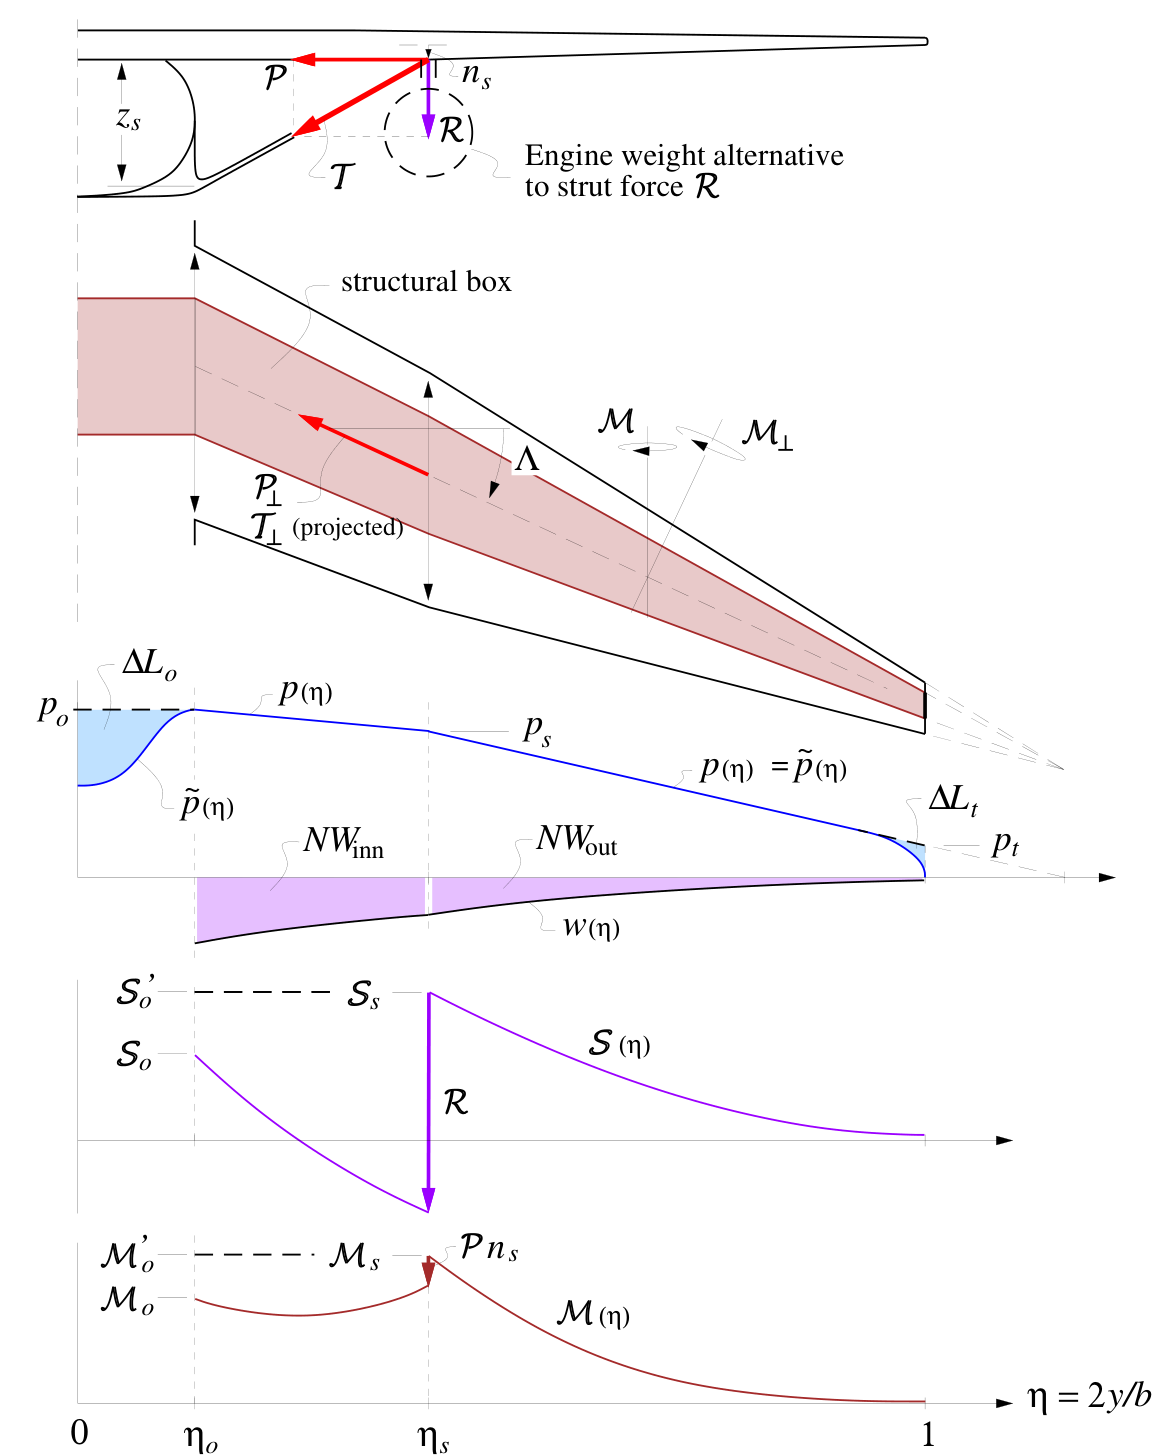
\includegraphics[width=4in]{../figures/nan-propagation/image1.png}
    \caption{Illustration of TASOPT's wing weight model, reproduced from Drela \cite{drela_tasopt_2010}. The model uses an Euler-Bernoulli beam model to compute shear and moment distribution, and accepts a relatively large set of geometric parameters as inputs.}
    \label{fig:nan-tasopt-wing-weight}
\end{figure}


For the purposes of this demonstration, the code implementation of this model is accessed through \emph{TASOPT.jl}, which is a transpilation of the original Fortran code into Julia performed by Prakash et al. \cite{tasopt_jl}. We aim to estimate the sparsity pattern of this function from within Python while accessing this model only through a Python-Julia interface, making this a true black-box function written in an entirely separate programming language.

\subsection{Sparsity Evaluation}

The first step in the NaN-propagation technique is to obtain a representative input. In the context of an optimization problem, the initial guess provides a natural choice:

\begin{figure}[H]
    \centering
    \includegraphics[page=2, width=5in]{../figures/nan-propagation/cropped.pdf}
\end{figure}

Next, we create a set of ``contaminated'' inputs, essentially by merging this input with one-hot encoded NaN values:

\begin{figure}[H]
    \centering
    \includegraphics[page=3, width=5in]{../figures/nan-propagation/cropped.pdf}
\end{figure}

Finally, we evaluate the black-box function at each of these contaminated inputs, and observe which outputs become NaN. For example, the output for one such contaminated input is shown below:

\begin{figure}[H]
    \centering
    \includegraphics[page=4, width=5in]{../figures/nan-propagation/cropped.pdf}
\end{figure}

This simple procedure yields the complete bipartite graph of which inputs and outputs are linked, and this can be interpreted as a sparsity pattern. For the demonstration case study, the sparsity pattern is shown in Figure \ref{fig:nan-jacobian}.

\begin{figure}[H]
    \centering
    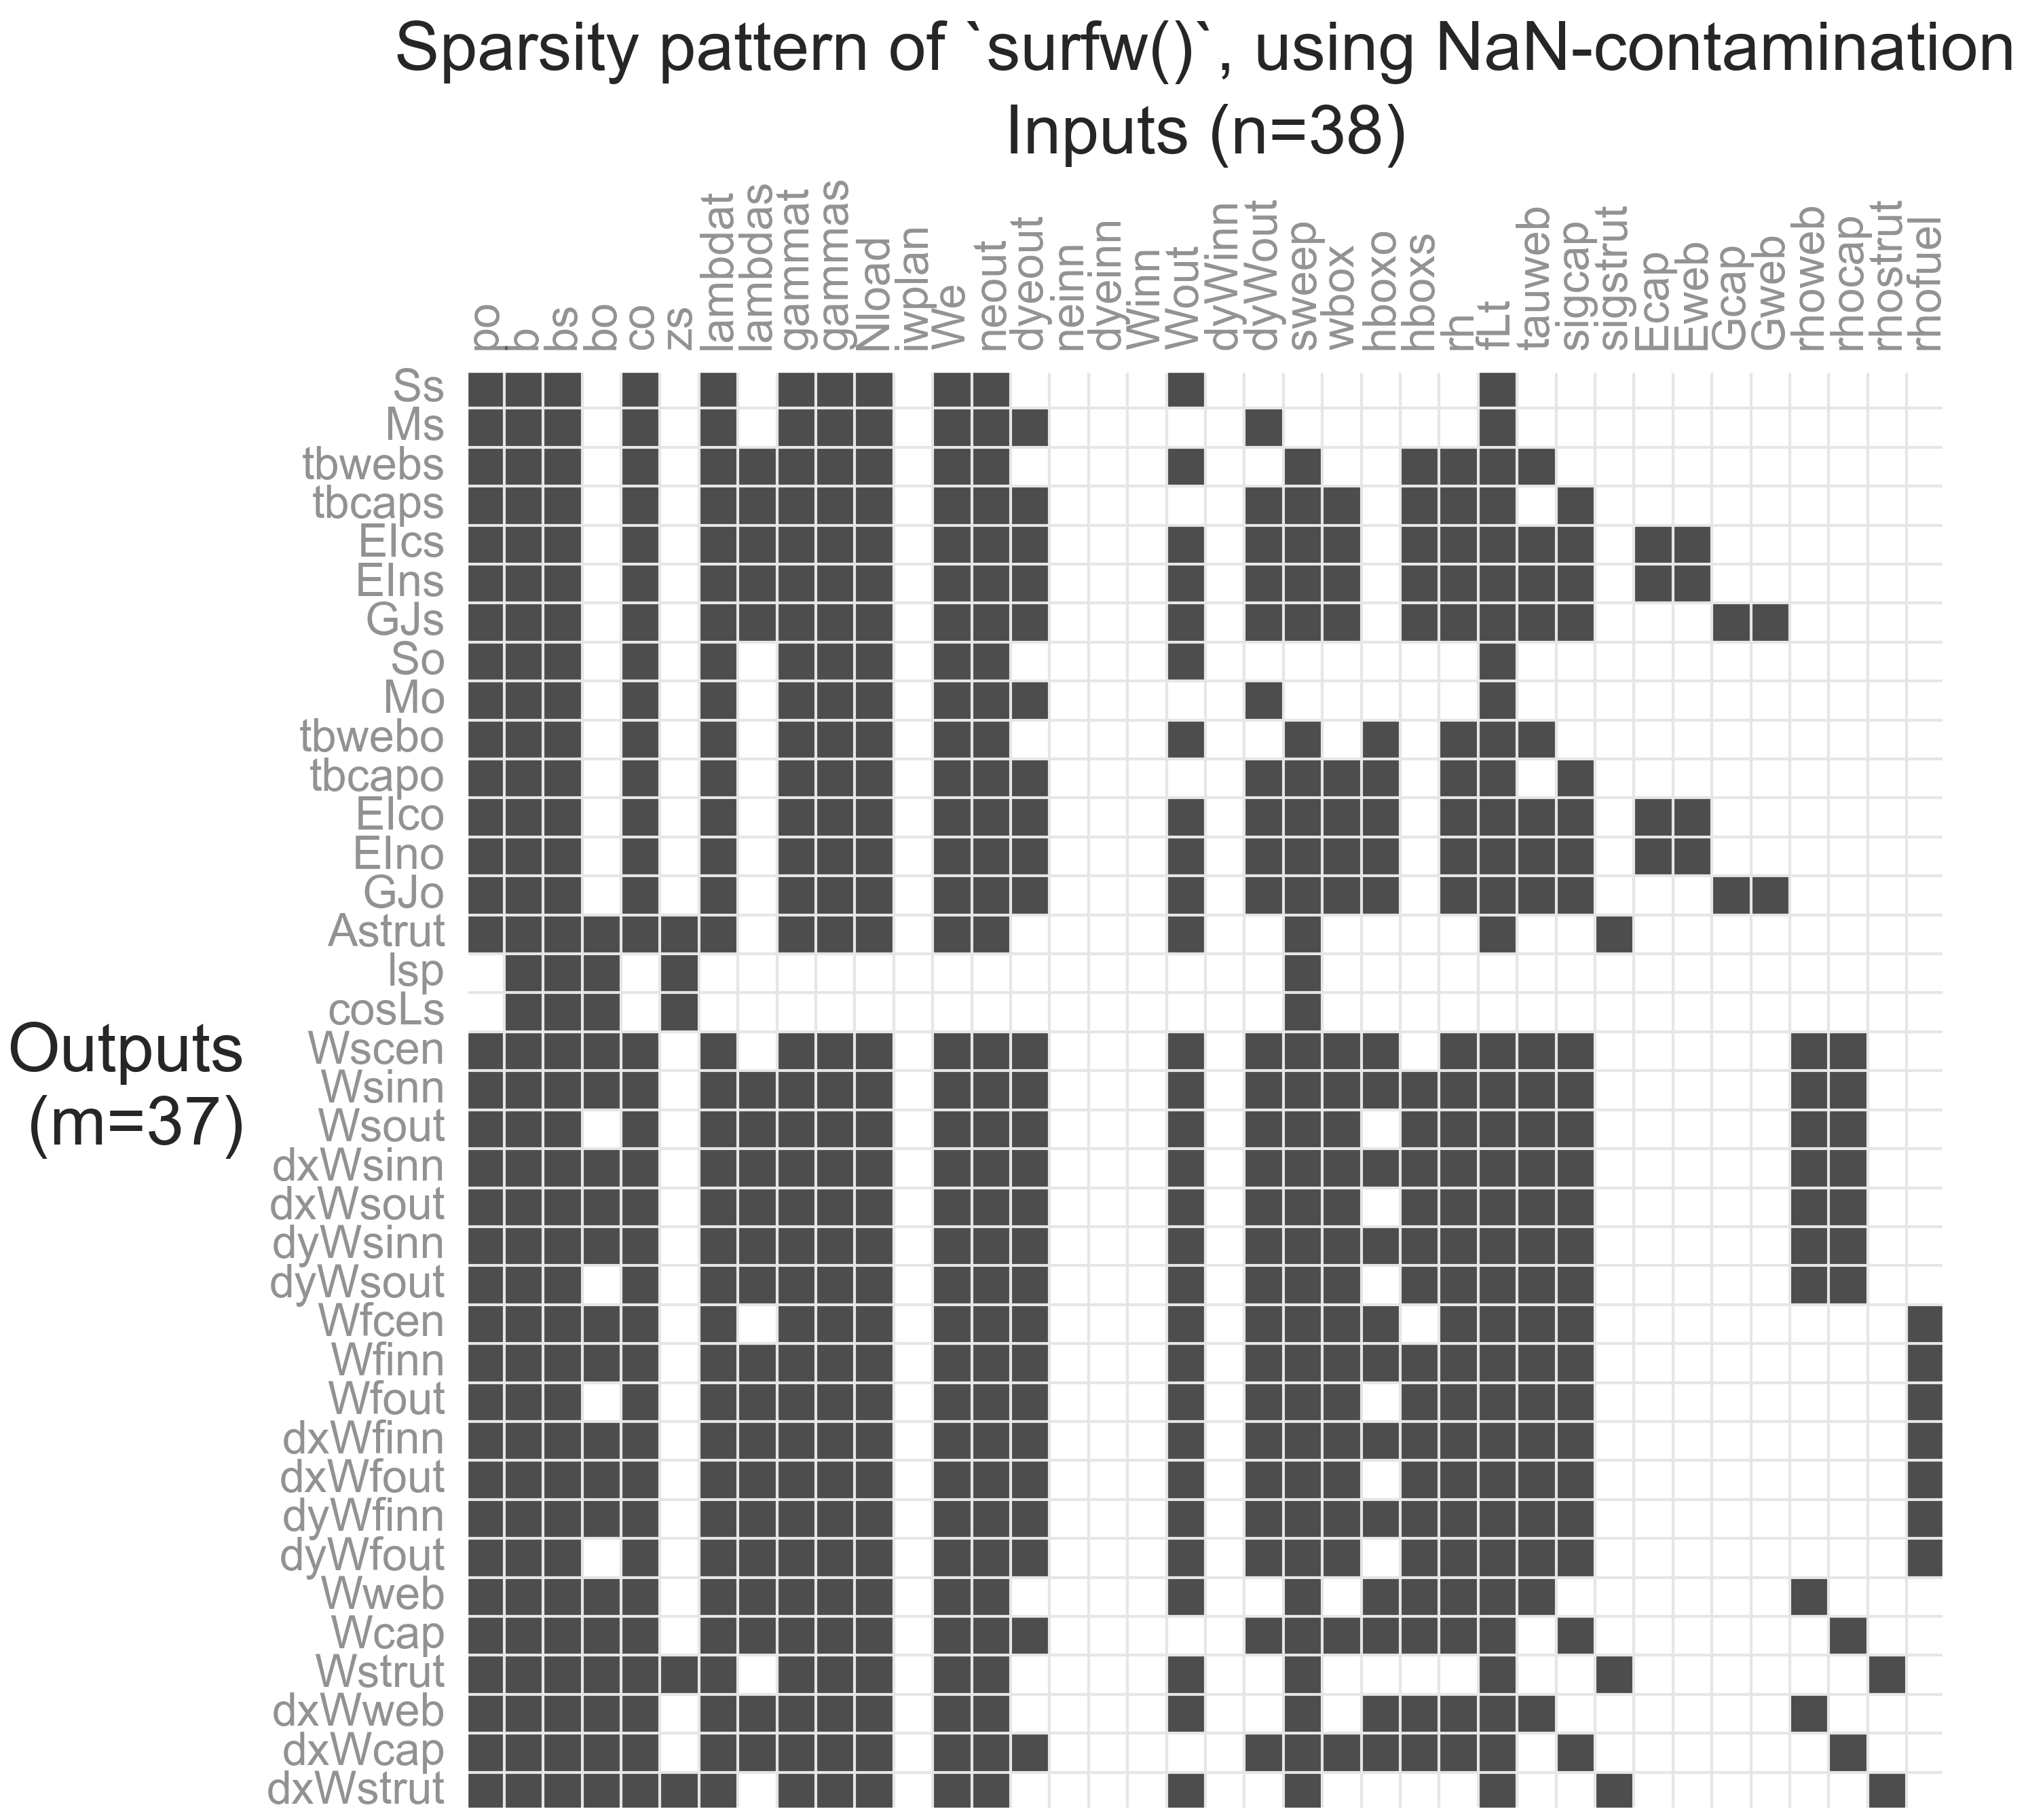
\includegraphics[width=6in]{../figures/nan-propagation/image2-crop.png}
    \caption{Sparsity pattern of the TASOPT wing weight model, estimated using NaN propagation. In this visualization, gray squares indicate nonzero entries in the Jacobian, }
    \label{fig:nan-jacobian}
\end{figure}

A key result is that this NaN-contamination technique eliminates the possible false-negative failure mode of coincidental zero gradients that can occur with existing gradient-based methods. Consider the example case discussed in Section \ref{sec:nan-existing-methods}, where the sparsity of the function $f(x) = x^2$ is traced at $x=0$. Here, a NaN-contamination technique will still detect the dependency between $x$ and $f(x)$, while existing methods will not. Because the potential consequence of a false-negative is so large, this represents a significant advantage over existing methods.

\subsection{Jacobian Compression}
\label{sec:nan-jacobian-compression}

This sparsity pattern can be used to enable gradient computation accelerations via simultaneous evaluation. More precisely, this involves Jacobian compression across columns, since the gradients of this black-box will later be obtained with finite-differencing (``forward-mode''-like behavior). Briefly, the steps to achieve this are:

\begin{enumerate}
    \item Convert the sparsity pattern into an undirected graph representation where each node corresponds to an input (i.e., a column in Figure \ref{fig:nan-jacobian}), and the presence of each edge indicates that the corresponding pair of inputs has overlapping sparsity. Conveniently, the adjacency matrix of this graph can be obtained by computing the Gramian of the sparsity pattern. If the sparsity pattern is represented as the binary matrix $S$, then the adjacency matrix of the graph is the binary matrix $S^T S \neq 0$.
    \item Apply a vertex coloring algorithm to this graph. This is a well-studied problem with many efficient approximate algorithms available \cite{kubale_graph_2004}.
\end{enumerate}

Visually, the result of this process can be shown with the compressed Jacobian of Figure \ref{fig:nan-jacobian-compressed}. Here, several columns show a combination of multiple inputs, and gradients with respect to these inputs can be safely computed simultaneously due to structural independence. The improvement in gradient computation speed is case-dependent, but in this demonstration, a reduction from 38 inputs to 25 effective inputs is achieved. Because gradient computation runtime scales linearly with the number of inputs in a finite-difference (or complex-step) context, this means that all future gradient calculations are roughly $38/25 \approx 1.52$x faster than a dense Jacobian construction.

\begin{figure}[H]
    \centering
    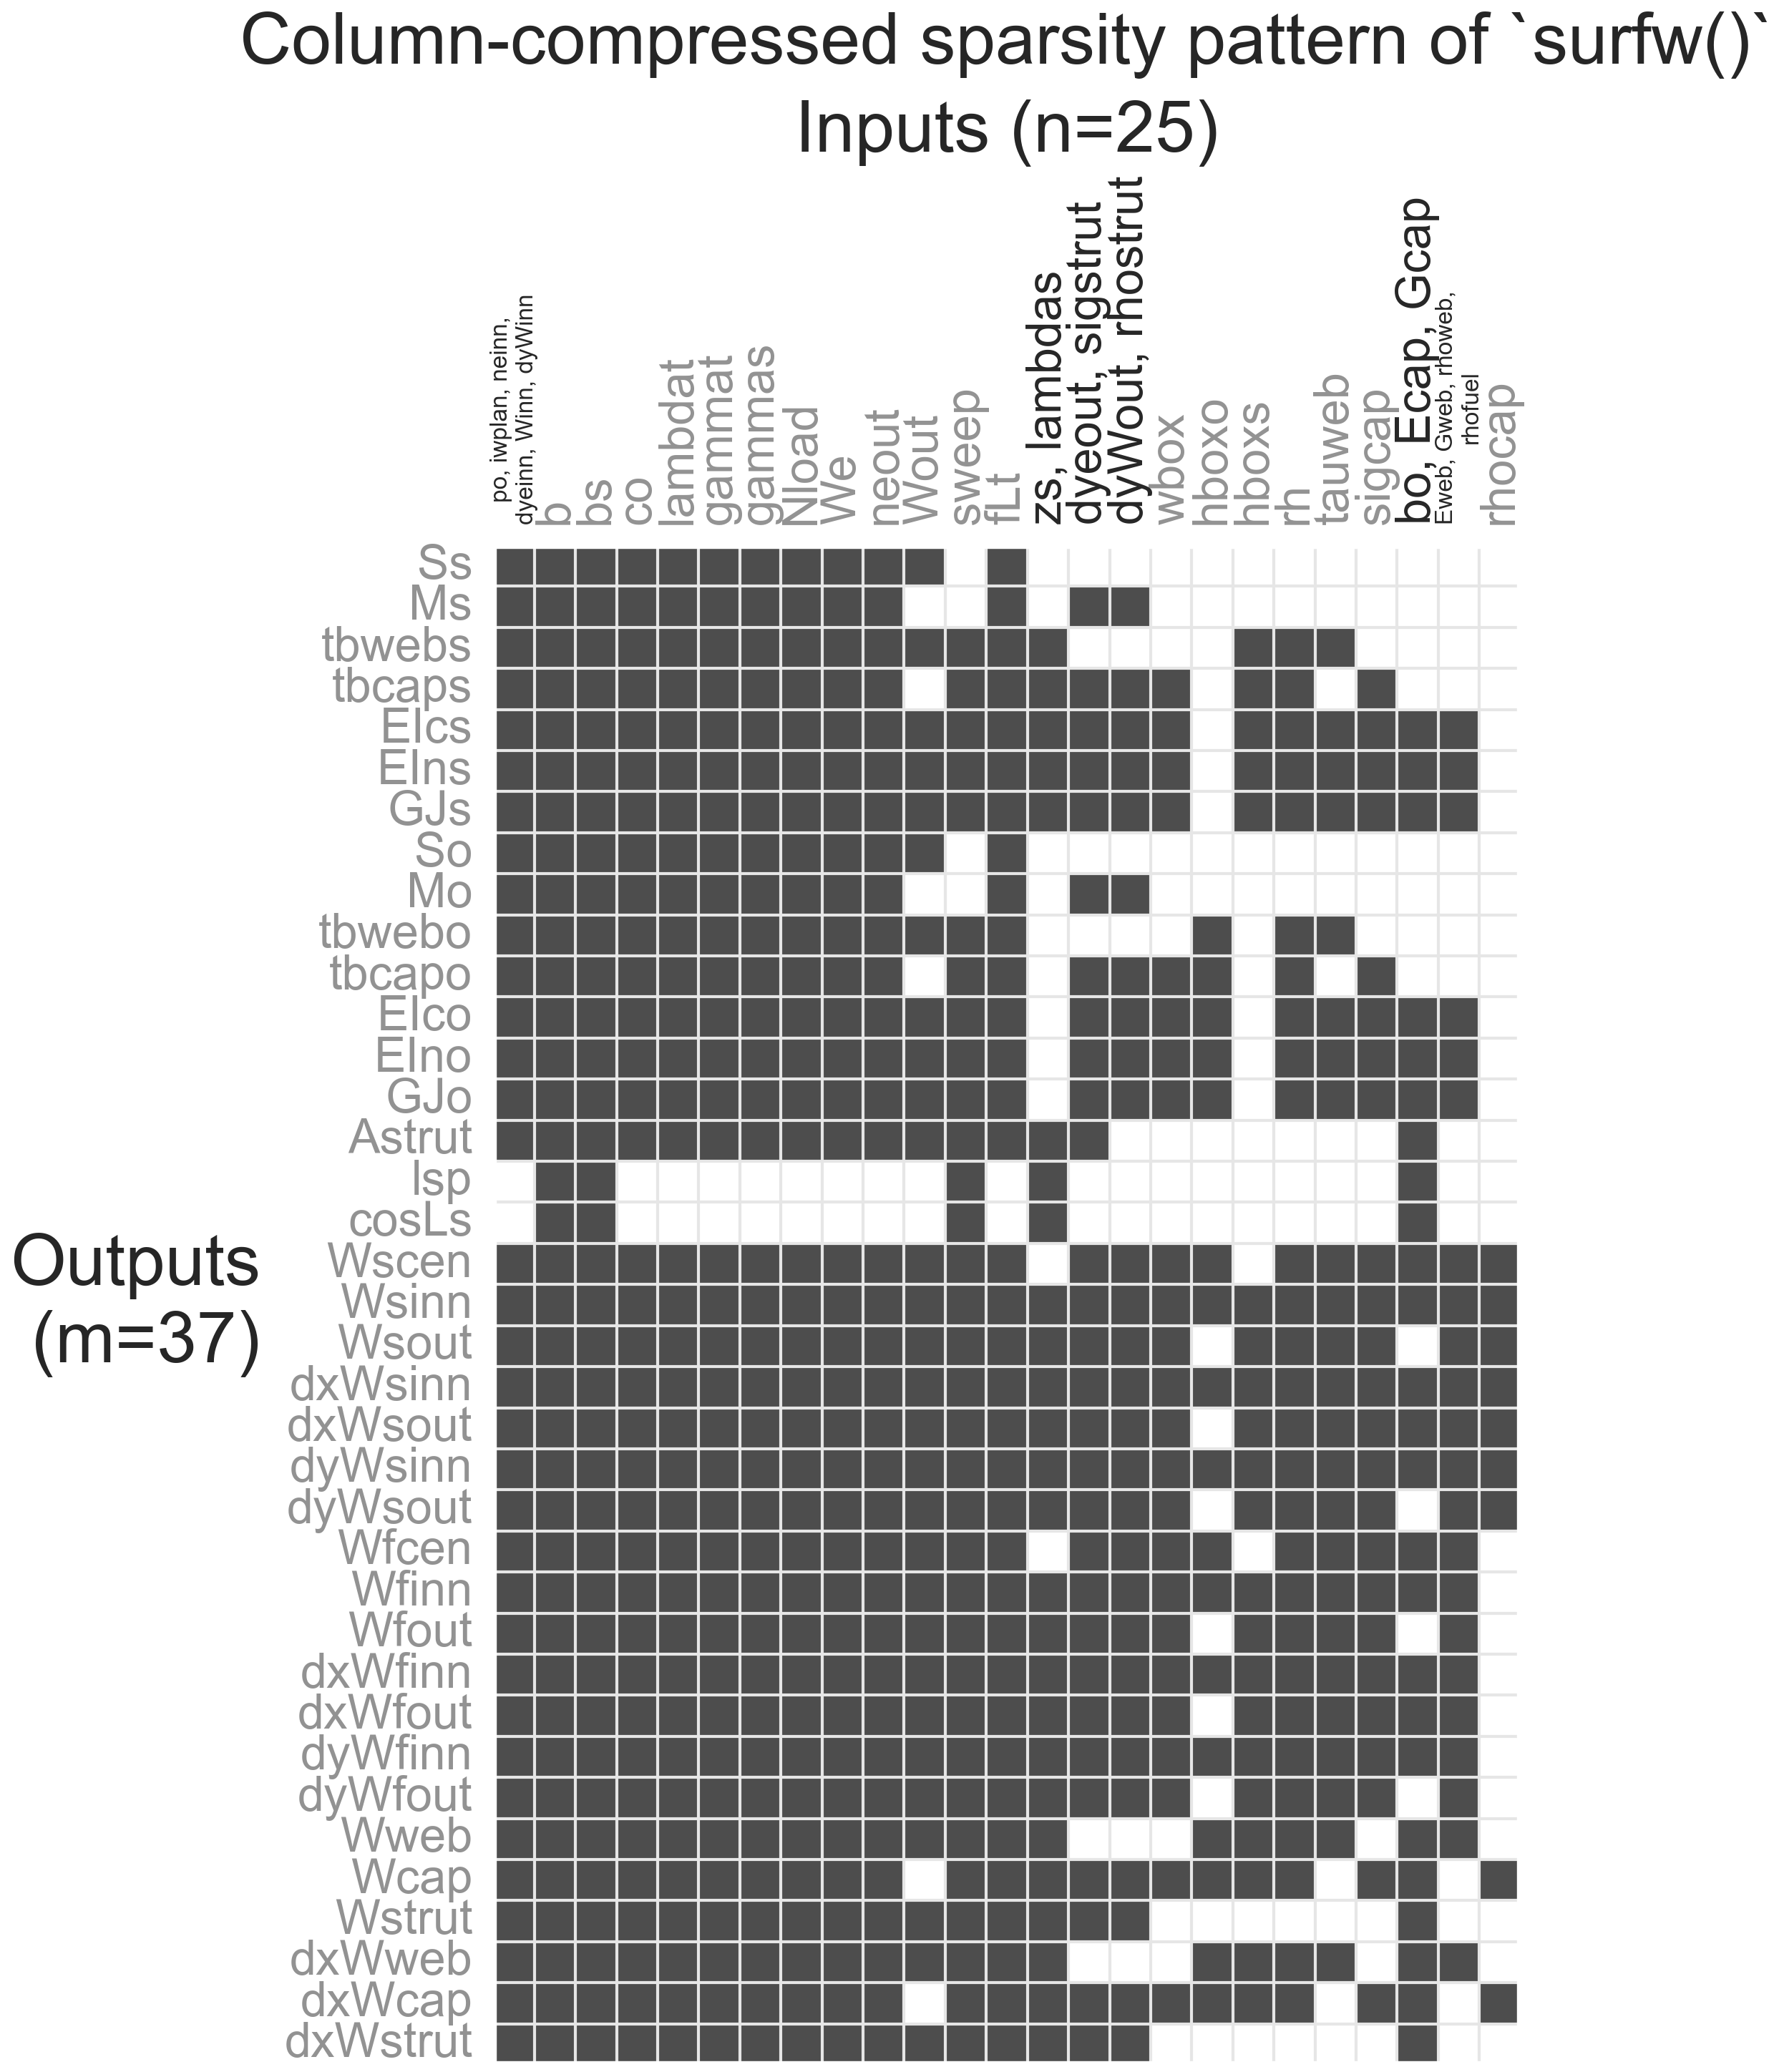
\includegraphics[width=5in]{../figures/nan-propagation/image3-crop.png}
    \caption{Compressed sparsity pattern of the TASOPT wing weight model, obtained by applying vertex coloring to the sparsity pattern of Figure \ref{fig:nan-jacobian}.}
    \label{fig:nan-jacobian-compressed}
\end{figure}


\section{Speed Considerations}

This gradient acceleration comes at a small upfront computational cost, since performing the sparsity trace requires a number of function evaluations equal to the number of inputs. This is true for both existing methods (described in Section \ref{sec:nan-existing-methods}) and for NaN-contamination. This cost is nearly always worthwhile in the context of design optimization: for the TASOPT wing model, a sparsity trace ``pays for itself'' in runtime if the subsequent optimization process requires more than three gradient evaluations.

In some cases, the runtime of a NaN-contamination-based sparsity trace will be essentially equal to that of standard finite-difference-based sparsity estimate. Intuitively, this makes sense, because both approaches require the same number of black-box function evaluations. However, in other cases, NaN-contamination can actually be significantly faster due to operator \textit{short-circuiting}. In this context, short-circuiting refers to operators that will check for NaN input values before performing computation; if any are found, the computation is skipped and a NaN is immediately returned instead. Programming languages and math libraries vary widely in whether and how they implement NaN-short-circuiting, so the magnitude of this potential speed-up is highly case-dependent.

\section{Potential Limitations}

While NaN-contamination eliminates a notable false-negative failure mode compared to existing methods, it also has several possible pitfalls that merit discussion. Some of these pitfalls are shared with existing methods, while others are unique to this technique.

\subsection{Mathematical False-Positives}

One limitation of NaN-contamination is that it can introduce new false-positive failure modes. To illustrate one possible mechanism, consider a scenario where we attempt to NaN-propagate through a black-box function written in code as $f(x)= x - x$. If $x$ is real-valued, then the correct result of a sparsity trace is that the input $x$ and the output $f(x)$ are structurally unrelated. However, a NaN-contamination technique will indicate a possible dependency here, as NaN values do not subtractively cancel. In contrast, existing gradient-based methods will correctly identify independence. More generally, this kind of false-positive can occur in any function where self-cancellation leads to structural independence, such as $f(x) = \sin(x)^2 + \cos(x)^2$ or $f(x) = x^0$.

In some ways, this false-positive is an unavoidable result of the same properties that allow NaN-contamination to eliminate false negatives due to coincidental zero gradients. In theory, global knowledge of this function as a computational graph could allow this self-cancellation to be detected and avoided. However, this would require a level of introspection that is fundamentally incompatible with the black-box nature of the function.

\subsection{Internal NaN Handling}

NaN-contamination is not compatible with all black-box functions. In particular, black-box functions that internally handle NaN values may not allow propagation. Most commonly in this scenario, the function will instead raise an error and halt the computation. This behavior is easily and immediately detected, and the sparsity detection routine can fall back to existing gradient-based methods in these cases.

A more serious false-negative failure mode can occur if the program actively overwrites NaN outputs without raising an error, as this can result in false negatives in the sparsity trace. Fortunately, this overwriting behavior is quite rare in engineering analysis code today. The main way this can occur is if the black-box code returns special flag values (sometimes called \emph{magic numbers}) to signal invalid computation, though this is generally considered an anti-pattern and avoided in numeric code. Even in code that has this overwriting behavior upon seeing a NaN result, most codes will at least raise a warning to the user.

Another possible false-positive failure mode can occur if operators within the black-box are overly aggressive about propagating NaN values. For example, consider a simple matrix-vector multiplication of the form $\vec{f}(\vec{x}) = \mat{A} \vec{x}$. If a single element of the matrix $A_{ij}$ is NaN, this should result in a single NaN output $f_i$, while the remaining elements are unaffected. Most programming languages and math libraries (e.g., NumPy, Julia) implement this behavior, allowing an accurate sparsity trace. However, some older libraries may aggressively contaminate and yield a NaN output for the entire output vector, which effectively results in false-positives.

\subsection{Branching Code Execution}
\label{sec:nan-bce}

Finally, branching code execution remains a challenge for NaN-contamination-based sparsity tracing, just as it is with existing methods. An example of this can be shown with the wing weight demonstration problem described in Section \ref{sec:nan-demo}. Here, the input variable \texttt{iwplan} is essentially an enumerated type that controls the wing configuration. Specifically:

\begin{itemize}[noitemsep]
    \item \texttt{iwplan = 0} or \texttt{iwplan = 1} corresponds to a cantilever wing without a strut.
    \item All other values of \texttt{iwplan} correspond to a wing with a strut.
\end{itemize}

Perhaps unsurprisingly, the sparsity pattern of the function becomes materially different if the wing configuration is changed by adding a struct. This is shown in Figure \ref{fig:nan-jacobian-branching}.

\begin{figure}[H]
    \centering
    \begin{subfigure}{0.49\textwidth}
        \centering
        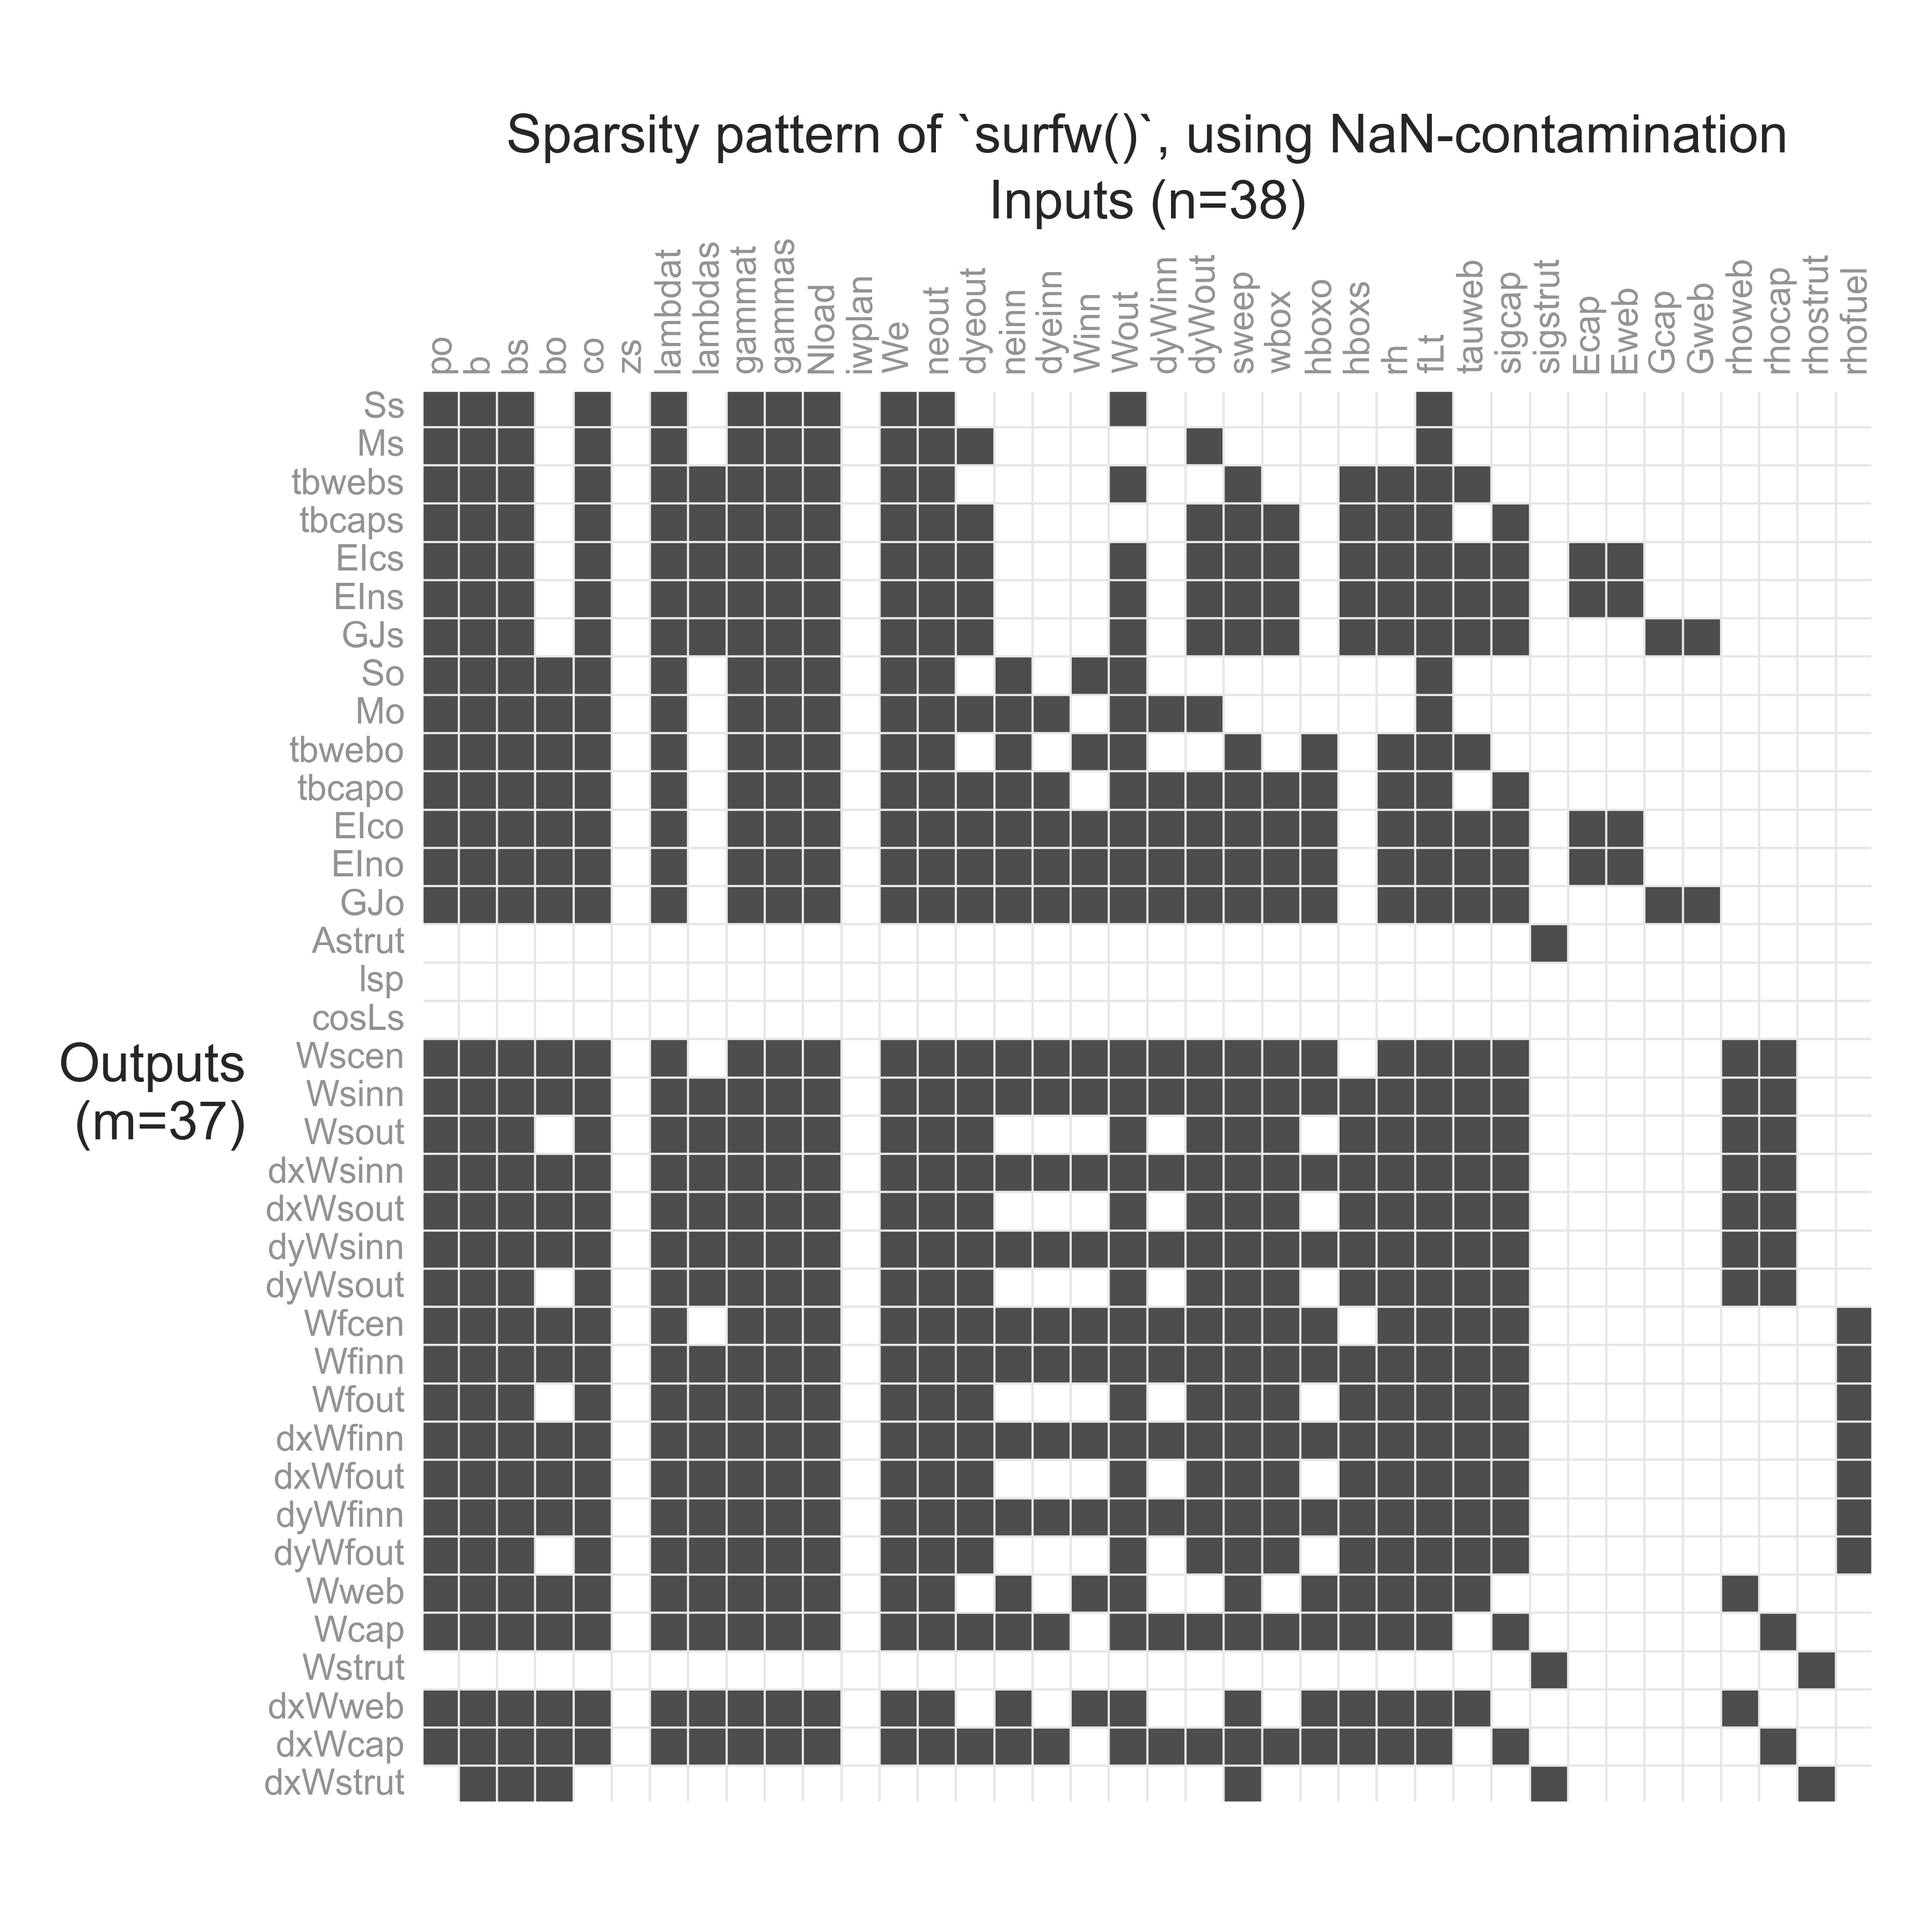
\includegraphics[width=\textwidth]{../figures/nan-propagation/image4.png}
        \caption{Without strut (\texttt{iwplan = 1})}
    \end{subfigure}
    \begin{subfigure}{0.49\textwidth}
        \centering
        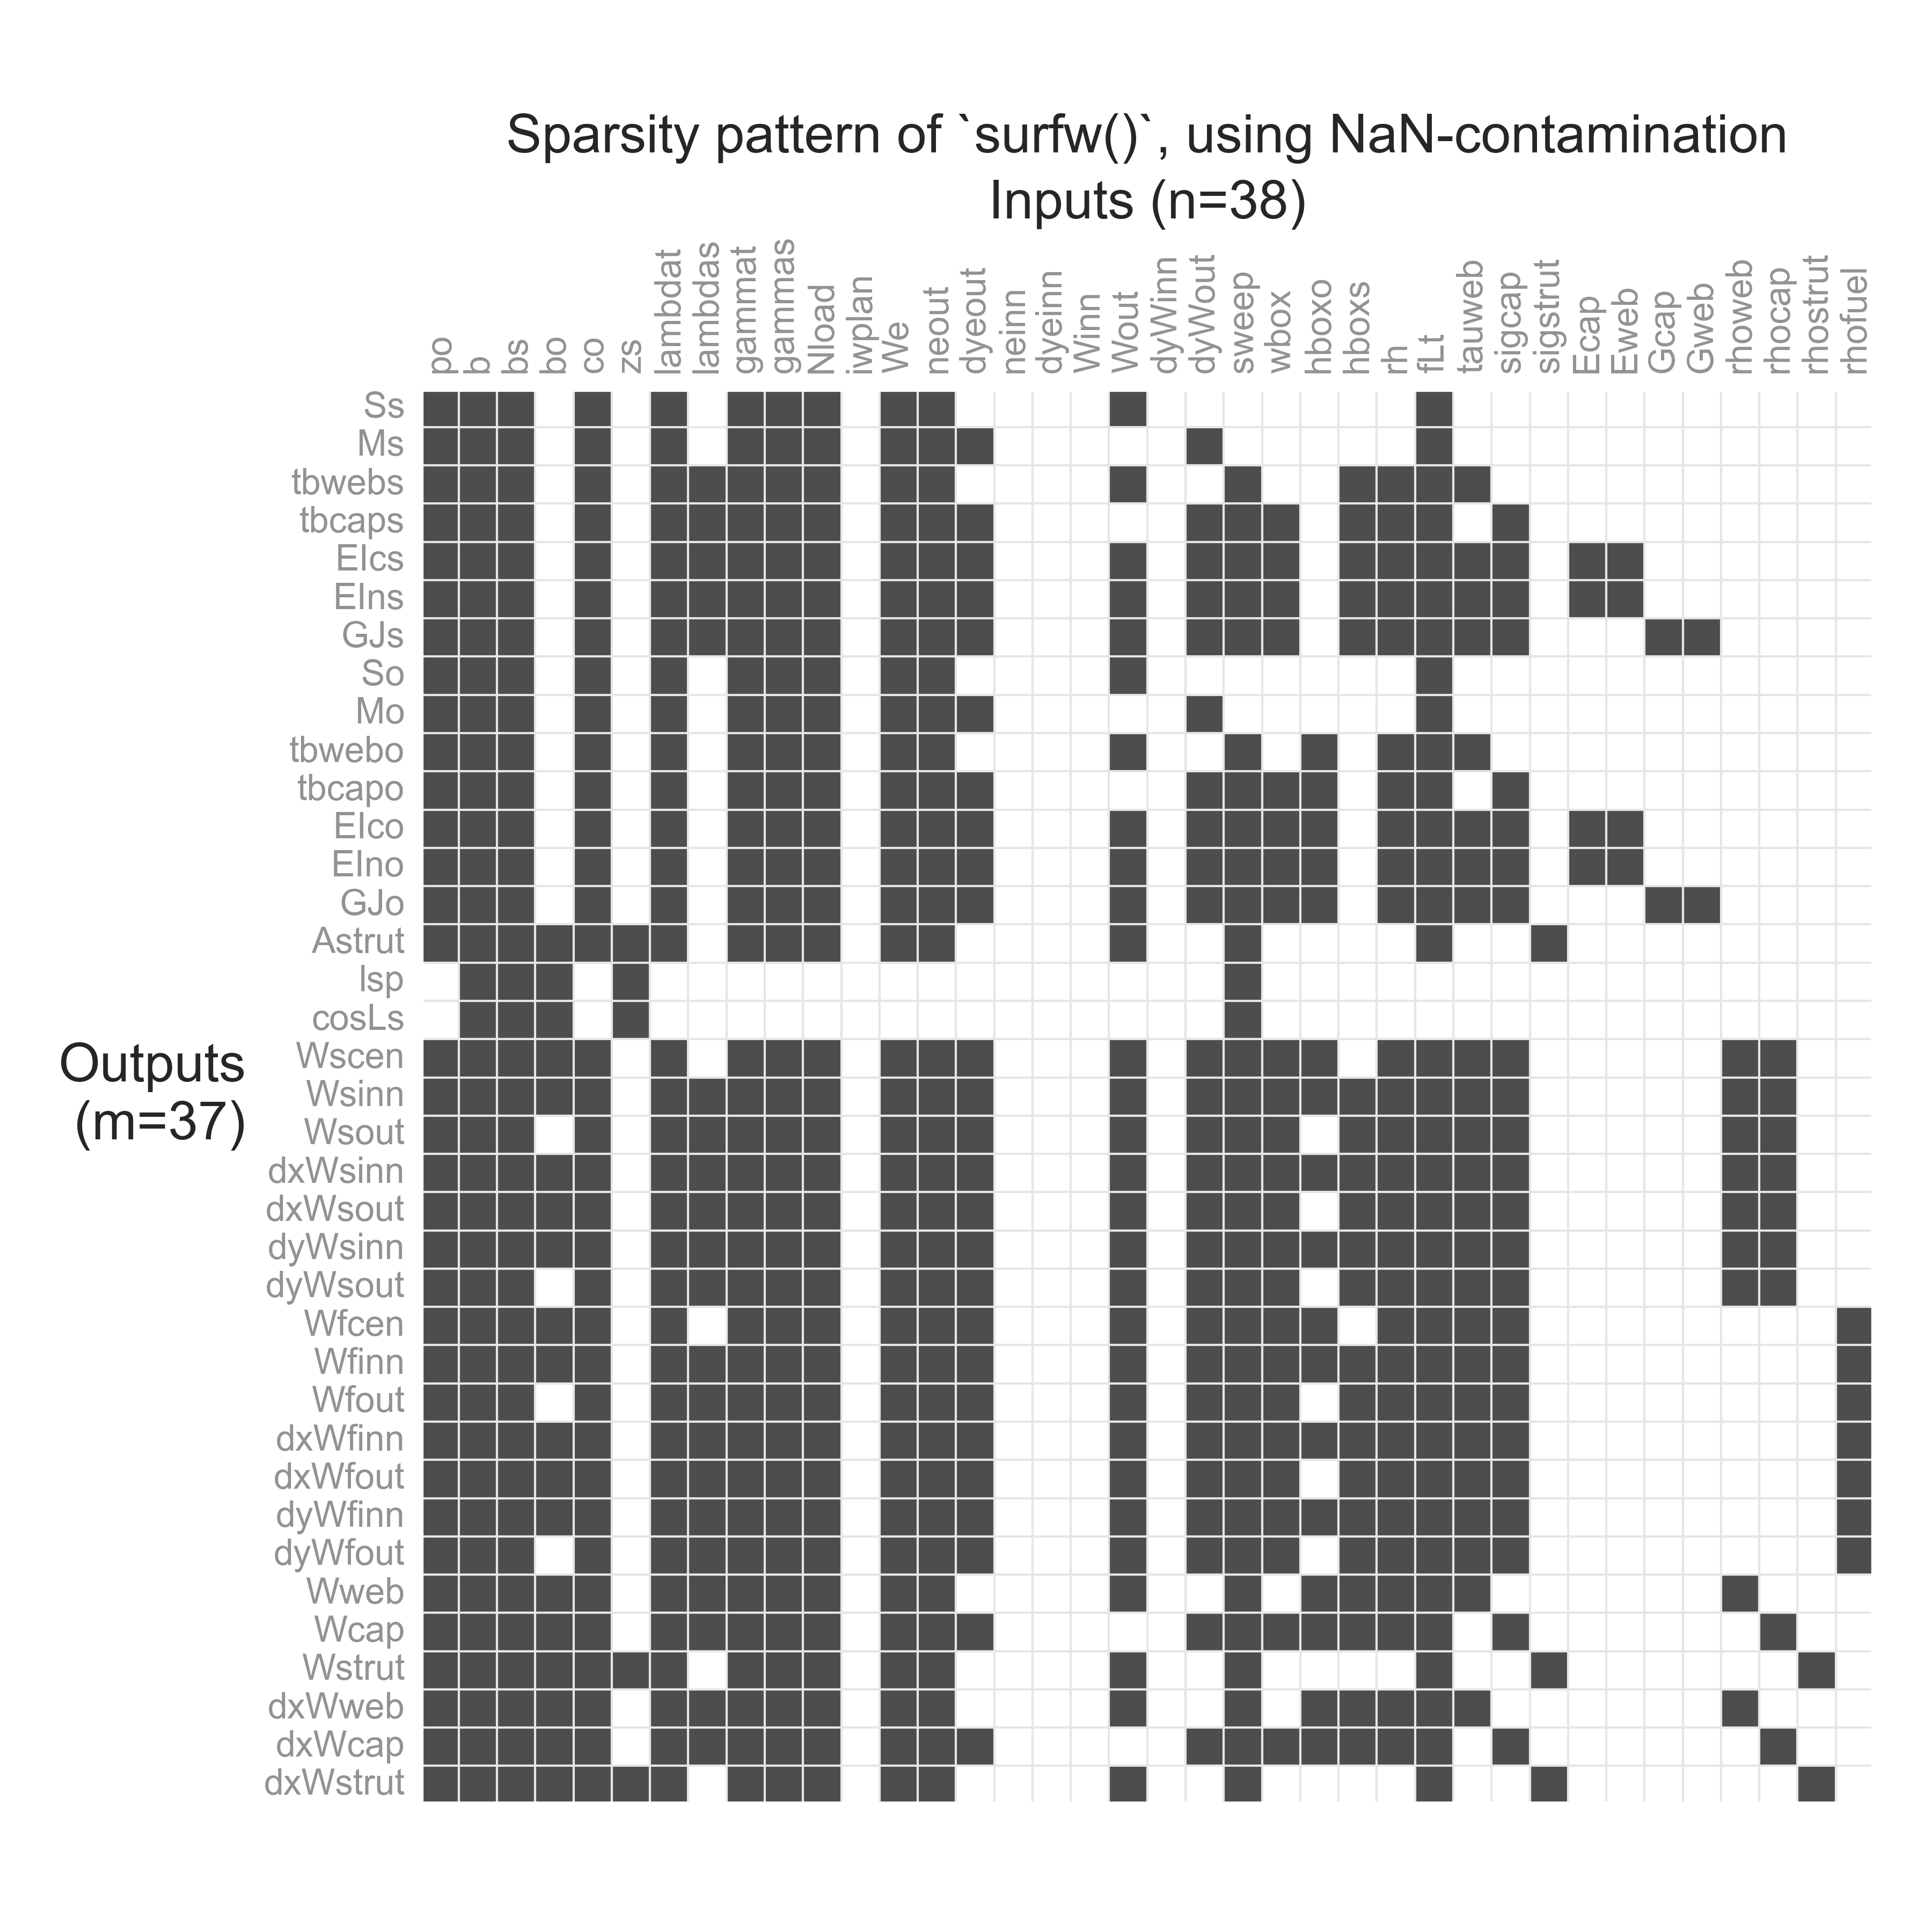
\includegraphics[width=\textwidth]{../figures/nan-propagation/image5.png}
        \caption{With strut (\texttt{iwplan = 2})}
    \end{subfigure}
    \caption{Sparsity pattern of the TASOPT wing weight model, estimated using NaN contamination, as the presence of a strut is varied by changing an input variable.}
    \label{fig:nan-jacobian-branching}
\end{figure}

With respect to branching code execution, NaN-contamination based strategies may have an advantage over existing methods due to the presence of \emph{static conditional} operators. These operators, which are offered in several math libraries, allow for conditional statements to be represented at an \emph{operator} level rather than a \emph{language} level. (In many languages, this is a ternary operator with a name similar to \texttt{ifelse}, \texttt{cond}, or \texttt{where}.) In such operators, both branches of the conditional are evaluated, yet only one is returned. This contrasts with language-level conditionals (e.g., traditional \texttt{if} statements), where the actual path of code execution changes. In some math libraries (e.g., CasADi) static conditionals allow NaNs to propagate through regardless of the condition—if either branch evaluates to NaN, the result is a NaN even if the NaN branch would not ordinarily be taken. Because of this, NaN-contamination-based sparsity tracing can potentially handle branching code execution better than existing options, depending on the math library used by the black box.

\section{Mitigating Branching Code Execution for Black-Box Engineering Analyses}

While branching code execution inherently poses problems for black-box sparsity tracing in the general sense, there are heuristic strategies that can be used to improve performance in practical cases. In particular, we look at strategies that tend to work well specifically in the context of engineering analysis code. In these cases, code branching often corresponds to variables that either change the design configuration or the mode of an analysis. The \texttt{iwplan} variable discussed in Section \ref{sec:nan-bce} is an example of this. With this in mind, we can make two observations specific to engineering analysis code that can be exploited.

First, inputs that trigger branching code execution -- collectively, ``flag inputs'' -- are often represented as discrete data types (e.g., integers, booleans, or strings) rather than continuous types (floating-point values). Because of this, knowledge of the input data types would allow some inferences to be drawn about which inputs are likely to trigger branching execution. In some cases, users may be able to manually mark flag inputs, either by leveraging domain knowledge or by inspecting known type-stable code\footnote{e.g., if the black-box function is written in a statically-typed language, and the user can view at least the function signature}. Of course, in the general case of a black-box function, this ability to inspect a function's type signature (either manually or dynamically) is not guaranteed. However, one possible option is to perform automatic type inference at runtime based on the types that constitute the initial guess.

Secondly, we can also take advantage of the fact that, in many cases, the value of flag inputs remains fixed during a single optimization study. For example, the design configuration may be kept fixed in a sizing study, or an analysis may only be run under certain assumptions. In such cases, the potential damage of a false negative is nullified, because the model is never evaluated on the other code branch.

One possible solution that takes advantage of both of these observations is to use a greedy approach. Concretely:

\begin{enumerate}
    \item Run an initial sparsity trace on the black-box model using the initial guess as the input.
    \item Every time a new value is observed on a discrete-typed input, re-run the sparsity trace.
    \item Take the result of this sparsity trace, and compute the union with all previously-observed sparsity patterns for this black-box model. Use this new sparsity pattern for Jacobian compression in subsequent evaluations.
\end{enumerate}

A visual illustration of this method is given in Figure \ref{fig:nan-bce-greedy}. Here, the sparsity pattern is iteratively refined as new values are observed on the discrete-typed input.

\begin{figure}[H]
    \centering
    \includegraphics[page=9, width=\textwidth]{../figures/nan-propagation/cropped.pdf}
    \caption{Illustration of a greedy algorithm for iteratively estimating the sparsity pattern of black-box models, in the presence of branching code execution. This approach is intended for use with engineering analysis models, and the process is applied to the example problem of Section \ref{sec:nan-demo}.}
    \label{fig:nan-bce-greedy}
\end{figure}

It should be emphasized that this algorithm is only a heuristic, and piecewise branching on continuous variables remains problematic. However, this strategy still offers substantial practical improvements over existing techniques that use a sparsity pattern purely based on Jacobian evaluation at the initial guess.


\section{Overall Comparison to Existing Methods}
\label{sec:nan-comparison}

In summary, the main advantage of the NaN-propagation technique is that it eliminates a key false-negative failure mode of existing gradient-based sparsity detection methods. To compare this more precisely, we can show a side-by-side comparison of the sparsity patterns obtained by each method for the TASOPT wing weight model. This is given in Figure \ref{fig:nan-comparison}. In this example, the initial guess used for Jacobian evaluation is taken from the TASOPT-supplied default for aircraft design optimization. Subfigure \ref{fig:nan-comparison-fd} reveals dozens of false negatives (marked as \textcolor{red}{\texttt{X}}) that are not captured by existing methods, but are detected with NaN-propagation. This clearly demonstrates the potential utility of NaN-propagation for sparsity-tracing black-box code functions.

\begin{figure}[H]
    \centering
    \begin{subfigure}{0.49\textwidth}
        \centering
        \includegraphics[page=10, width=\textwidth]{../figures/nan-propagation/cropped.pdf}
        \caption{Sparsity pattern obtained by NaN-propagation.}
    \end{subfigure}
    \begin{subfigure}{0.49\textwidth}
        \centering
        \includegraphics[page=11, width=\textwidth]{../figures/nan-propagation/cropped.pdf}
        \caption{Sparsity pattern obtained using existing finite-difference methods. All red \textcolor{red}{\texttt{X}} marks denote false negatives that are not captured by existing methods, but detected with NaN-propagation.}
        \label{fig:nan-comparison-fd}
    \end{subfigure}
    \caption{Comparison of sparsity patterns obtained by NaN-propagation and existing finite-difference methods for the TASOPT wing weight model. Existing methods lead to false negatives via coincidental zero gradients, which can lead to costly mistakes during Jacobian compression.}
    \label{fig:nan-comparison}
\end{figure}


\section{Advanced Strategies}

This chapter has introduced the core NaN-propagation technique, along with its benefits over existing methods and potential limitations. In this section, we introduce several advanced strategies that can be used to further improve the performance of NaN-propagation-based sparsity tracing.

\subsection{NaN Payload Encoding}

One possible extension is based on a recognition that not all NaN values are identical, and there are multiple unique binary representations that are interpreted as NaN values. Careful use of these values can essentially allow the encoding of additional information to aid sparsity tracing. To illustrate this, consider the binary representation of a single-precision (32-bit) floating-point NaN value, following the IEEE 754 standard \cite{ieee754}:

\newcommand{\pbit}[1]{\texttt{\textcolor{mydodgerblue}{#1}}} % Payload bit

\begin{equation*}
    \texttt{NaN = \textcolor{mydodgerblue}{x}111 1111 1\textcolor{mydodgerblue}{xxx xxxx xxxx xxxx xxxx xxxx}}
\end{equation*}


\begin{eqexpl}[20mm]
    \item {\texttt{0, 1}} bit values
    \item {\pbit{x}} \emph{any} bit (with the edge-case exception that not all trailing bits can be zero, or the value is interpreted as $\infty$)
\end{eqexpl}

Regardless of the value of the \pbit{x} bits, this value will be interpreted as a NaN. Therefore, single-precision NaN representations allow us to encode nearly 22 bits of information (as there are $2^{22} - 2$ unique NaN values) into the these \pbit{x} bits, which we call the \emph{payload}. In double-precision (64-bit) floating point arithmetic, which is more common in engineering analysis, this payload is even larger at nearly 51 bits.

Crucially, these unique NaN payloads are propagated through mathematical operations. Therefore, we can ``tag'' individual inputs with unique NaN payloads, and observe which payloads are present in the outputs. Because NaN values are no longer fungible, \emph{multiple columns of the sparsity pattern can be simultaneously traced within a single function evaluation}. This presents a novel and fundamental theoretical improvement in the time-complexity of black-box sparsity tracing, since the number of function evaluations can now be independent of the number of inputs.

A natural question to ask is how NaN values are propagated through dyadic operations—in cases where an operator receives multiple payload-encoded NaN values, it is not obvious what the payload of the output will be. In general, most programming languages and math libraries will simply propagate one of the two operands unmodified, and ignore the other. However, which operand is preferred varies. For example, in Python, the addition, subtraction, and multiplication operators propagate the first NaN operand, while the division and exponentiation operators propagate the second NaN operand.

Because of this effect, some care is needed to take advantage of NaN payload encoding. To demonstrate this, consider a dyadic black-box function of the form $f(x_1, x_2)$. Say we perform a sparsity trace by evaluating the function at $x_1=\texttt{NaN}_1$, $x_2=\texttt{NaN}_2$, with subscripts representing that these are uniquely identifiable $\texttt{NaN}$ values. If the output of function $f$ is $\texttt{NaN}_1$, this indicates that $f$ is surely a function of $x_1$, but the sparsity with respect to $x_2$ is unknown. Likewise, the opposite is true if the output is $\texttt{NaN}_2$. In such cases, the simultaneous column evaluations of the sparsity pattern can be thought to ``shadow'' one another, in that a sparsity ``hit'' on one column precludes receiving information about the other. Because of this \emph{shadowing effect}, the time complexity of NaN-contamination with payload encoding is not quite $\order(1)$, though it can still be better than the $\order(N)$ of existing approaches (discussed later). Regardless, the real benefit associated with payload encoding occurs when the output $f$ is a function of neither input, as this allows exclusion of both inputs from the sparsity pattern with a single function evaluation. At a high level, any strategy that allows us to gain information about multiple inputs will result in a speedup.

As the sparsity pattern is constructed using NaN-payload-encoding, there must be some means of selecting which combination of columns should be simultaneously evaluated next for sparsity tracing. Development of an efficient column selection algorithm is left as an area of future work. However, we offer some observations that may guide this development for the interested reader:

\begin{enumerate}
    \item During sparsity tracing, the state of the sparsity pattern needs to be stored as a trinary matrix with three possible states: \texttt{0} (no dependency), \texttt{1} (dependency), and \texttt{2} (unknown). Because of this unknown factor, any good algorithm is inherently probabilistic. This unknown factor is also why this algorithm is not simply a degenerate case of a graph coloring algorithm.
    \item A good algorithm likely needs some tracker of the belief state about the density of the sparsity pattern (i.e., the fraction of unknown entries that are likely to be dependent vs. independent). This is because the estimated density of the sparsity pattern is related to how many columns should be evaluated simulaneously. If we believe that the sparsity pattern is relatively dense, then fewer columns should be evaluated simultaneously, as the shadowing effect will be significant. Conversely, if the sparsity pattern is believed to be sparse, then we should be more aggressive about evaluating more columns simultaneously, since we may be able to gain more information per function evaluation.

    One possible way to implement this density belief state is to use a Bayesian approach, where the belief state is updated at every step based on the results of the previous function evaluations. The initial belief state could be an uninformative prior (e.g., a uniform distribution), or one could accept a user-supplied estimate. This approach has some flaws (e.g., assuming the sparsity of each entry is independent), but it presents a reasonable starting point.

    \item An algorithm that selects which combination of columns should be evaluated next is inherently a combinatorial optimization problems. These are notoriously slow to solve, in the general case. However, if the black-box function is slow to evaluate (as it often is, in the case of engineering analysis), it may be well worth it to solve this problem. There are also many strategies that could accelerate this combinatorial optimization problem in this context. These could include leveraging dynamic programming (since similar versions of this problem are solved sequentially), using heuristic methods (e.g., simulated annealing, genetic algorithms), or solving a continuous relaxation of this problem.

    As a practical matter, one possible objective function of this algorithm is to maximize the expected improvement in the sparsity pattern, given the current belief state—this is similar to Bayesian optimization, though here it is applied in a discrete setting. This objective function could be formulated by considering the amount of Shannon entropy gained by evaluating with each combination of column evaluations, accounting for the expected value of the shadowing effect and the current belief state over the density of the sparsity pattern.
    \item Best-case time complexity, as measured by the number of function evaluations, should be $\order(1)$. However, this is only true in the trivial case where the sparsity pattern is all-zeros and no shadowing occurs. A more realistic best-case time complexity is $\order(\log(N))$, where $N$ is the number of inputs. This best-case complexity occurs in the limit of low-density sparsity patterns (e.g., an all-diagonal sparsity pattern) that are amenable to recursive halving. A worst-case time complexity is $\order(N)$, in the case of a fully-dense sparsity pattern—this is identical to both existing methods and NaN-propagation without payload encoding.
\end{enumerate}


\subsection{Chunking}

Another novel proposed acceleration, which we term ``chunking'', seeds multiple adjacent elements of the input vector with NaN values simultaneously. This is similar to the multiple seeding associated with payload NaN encoding, but its inclusion here is meant to emphasize that some benefits can be achieved even without bit-hacking NaN values to make them uniquely identifiable.

As an example: if pairs of adjacent inputs are seeded, this has the benefit of halving the number of function calls, at the detriment of providing overly-conservative sparsity information\footnote{as one cannot determine which NaN input caused a given output to return NaN, so neither can be ruled out} (i.e., one with false positives). This exploits the fact that a conservative sparsity pattern can still provide some speedup during Jacobian compression, even if it is less than what might be achieved with a more accurate sparsity pattern.

It also exploits the fact that sparsity patterns of human-written code are not uniformly random. In particular, these sparsity patterns tend to have a high degree of locality (e.g., inputs at indices 3 and 4 are much more likely to share a similar sparsity pattern than inputs at indices 3 and 30). This locality is due to the fact that, in an engineering analysis with multiple submodules, humans tend to code submodule A in its entirety before implementing submodule B. Because of this, these chunked sparsity patterns using adjacent inputs can be surprisingly accurate approximations in practice.

Thus, chunking may offer significant speedups in engineering practice by exploiting typical problem structure; a computational analogy would be how an $A^*$ graph traversal algorithm outperforms Dijkstra's algorithm in practice despite identical worst-case complexity. This and other heuristics can significantly reduce the number of black-box function evaluations required to trace the sparsity pattern.

\section{Computational Reproducibility}
\label{sec:nan-reproducibility}

All source code used to generate example results in this chapter is publicly available at \url{https://github.com/peterdsharpe/nan-propagation}.
